\documentclass[a4paper]{arrowhead}

\usepackage[yyyymmdd]{datetime}
\usepackage{etoolbox}
\usepackage[utf8]{inputenc}
\usepackage{multirow}

\renewcommand{\dateseparator}{-}

\setlength{\parskip}{1em}

%% Special references
\newcommand{\fref}[1]{{\textcolor{ArrowheadBlue}{\hyperref[sec:functions:#1]{#1}}}}
\newcommand{\mref}[1]{{\textcolor{ArrowheadPurple}{\hyperref[sec:model:#1]{#1}}}}
\newcommand{\pdef}[1]{{\textcolor{ArrowheadGrey}{#1\label{sec:model:primitives:#1}\label{sec:model:primitives:#1s}\label{sec:model:primitives:#1es}}}}
\newcommand{\pref}[1]{{\textcolor{ArrowheadGrey}{\hyperref[sec:model:primitives:#1]{#1}}}}

\newrobustcmd\fsubsection[3]{
  \addtocounter{subsection}{1}
  \addcontentsline{toc}{subsection}{\protect\numberline{\thesubsection}function \textcolor{ArrowheadBlue}{#1}}
  \renewcommand*{\do}[1]{\rref{##1},\ }
  \Subsection*{
    \thesubsection\quad
    function
    \textcolor{ArrowheadBlue}{#1}
    (\notblank{#2}{\mref{#2}}{})
    \notblank{#3}{: \mref{#3}}{}
  }
  \label{sec:functions:#1}
}
\newrobustcmd\msubsection[2]{
  \addtocounter{subsection}{1}
  \addcontentsline{toc}{subsection}{\protect\numberline{\thesubsection}#1 \textcolor{ArrowheadPurple}{#2}}
  \subsection*{\thesubsection\quad#1 \textcolor{ArrowheadPurple}{#2}}
  \label{sec:model:#2} \label{sec:model:#2s} \label{sec:model:#2es}
}
%%

\begin{document}

%% Arrowhead Document Properties
\ArrowheadTitle{Service Registry Core System}
\ArrowheadType{System Design Description}
\ArrowheadTypeShort{SysDD}
\ArrowheadVersion{4.4.0}
\ArrowheadDate{\today}
\ArrowheadAuthor{Tamás Bordi}
\ArrowheadStatus{RELEASE}
\ArrowheadContact{tbordi@aitia.ai}
\ArrowheadFooter{\href{www.arrowhead.eu}{www.arrowhead.eu}}
\ArrowheadSetup
%%

%% Front Page
\begin{center}
  \vspace*{1cm}
  \huge{\arrowtitle}

  \vspace*{0.2cm}
  \LARGE{\arrowtype}
  \vspace*{1cm}

  %\Large{Service ID: \textit{"\arrowid"}}
  \vspace*{\fill}

  % Front Page Image
  %\includegraphics{figures/TODO}

  \vspace*{1cm}
  \vspace*{\fill}

  % Front Page Abstract
  \begin{abstract}
    This document provides system design description for the \textbf{Service Registry Core System}.
  \end{abstract}

  \vspace*{1cm}

%   \scriptsize
%   \begin{tabularx}{\textwidth}{l X}
%     \raisebox{-0.5\height}{
\includegraphics[width=2cm]{figures/artemis_logo}} & {ARTEMIS Innovation Pilot Project: Arrowhead\newline
%     THEME [SP1-JTI-ARTEMIS-2012-AIPP4 SP1-JTI-ARTEMIS-2012-AIPP6]\newline
%     [Production and Energy System Automation Intelligent-Built environment and urban infrastructure for sustainable and friendly cities]}
%   \end{tabularx}
%   \vspace*{-0.2cm}
 \end{center}

\newpage
%%

%% Table of Contents
\tableofcontents
\newpage
%%

\section{Overview}
\label{sec:overview}
\color{black}
This document describes the Service Registry Core System, which exists to enable service discovery in a Eclipse Arrowhead Local Cloud (LC). In Section \ref{sec:implementation}, we describe implementation details of the system. In Section \ref{sec:services}, we summarize the services produced by the system.

\newpage

\section{Implementation}
\label{sec:implementation}

\subsection {Implementation language and tools}

\begin{itemize}
\item \emph{Programming Language:} \textbf{Java 11}
\item \emph{Programming Framework:} \textbf{Spring-Boot 2.1.5}
\item \emph{Building Tool:} \textbf{Maven 3.5+}
\item \emph{Database Management System:} \textbf{MySQL 5.7}
\item \emph{State:} \textbf{Stateful}
\end{itemize} 

\subsection {Functional properties implementation}

\subsubsection{Database structure}

Implementation of data storage functionality was done as described by Figure 1.

\begin{figure}[h!]
  \centering
  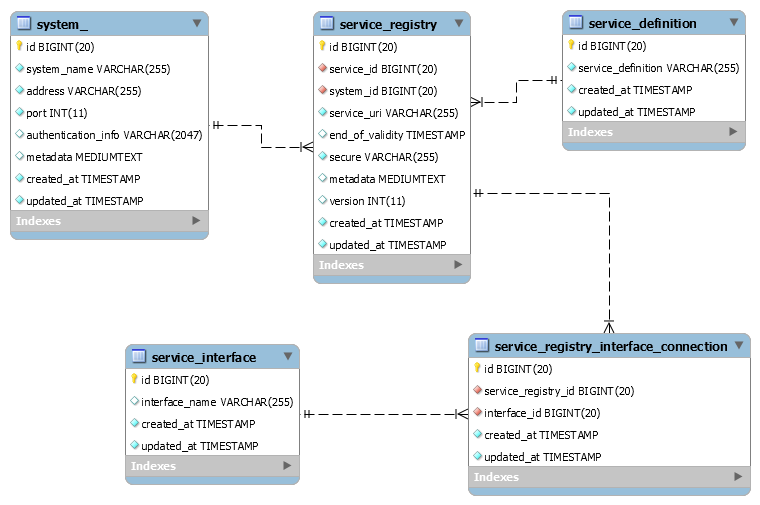
\includegraphics[width=\textwidth]{figures/serviceregistry_database_model}
  \caption{
    Database model of Service Registry Core System.
  }
  \label{fig:model_overview}
\end{figure}

\clearpage

\subsubsection{Configuration}
The system configuration properties can be found in the \texttt{application.properties} file which is located at \texttt{src/main/resources} folder.

\textit{Note:} During the build process this file is going to be built into the executable jar, but also going to be copied next to the jar file. Any modification in the configuration file located next to the executable jar file will overide the built in configuration property value.

\begin{itemize}
    \item \textbf{ping\_scheduled}
  
    If 'true' the service providers will be pinged in a fixed time interval and service offerings will be removed where the provider was not available.
    
    \item \textbf{ping\_timeout}
  
    How much time the system should wait for the ping response (in milliseconds).
    
    \item \textbf{ping\_interval}
  
    How frequently should the ping happen, in minutes.
    
    \item \textbf{ttl\_scheduled}
  
    If 'true' the service offerings will be automatically removed, where the endOfValidity timestamp field is in the past, meaning the offering expired.
    
    \item \textbf{ttl\_interval}
  
    How frequently the database should be checked for expired services, in minutes.
    
    \item \textbf{use\_strict\_service\_intf\_name\_verifier}
  
    Interface names has to follow this format \texttt{PROTOCOL-SECURITY-FORMAT}, where security can be \texttt{SECURE} or \texttt{INSECURE} and protocol and format must be a sequence of letters, numbers and underscore. A regexp checker will verify that. If this setting is set to true then the \texttt{PROTOCOL} and \texttt{FORMAT} must come from a predefined set.
    
    \item \textbf{use\_strict\_service\_definition\_verifier}
  
    If 'true', service definitions has to follow these rules: They only contains letters (english alphabet), numbers and dash (-), and have to start with a letter (also cannot end with dash).
    
    \item \textbf{use\_network\_address\_detector}
  
    If 'true', address detection from HttpServletRequest will be performed at the time of systems and service registration/unregistration.
    
    \item \textbf{filter\_proxy\_addresses}
  
    Comma separated list representing the possible proxy servers like load-balancer etc... before ServiceRegistry.
    
    \item \textbf{allow\_self\_addressing}
  
    If 'true', the registration of systems with self-addressing IPv4, IPv6 and no-type addresses are allowed. In case of self-addressing addresses the IP packets cannot be directed from one device to another.
    
    \item \textbf{allow\_non\_routable\_addressing}
  
    If 'true', the registration of systems with non-routable IPv4 and IPv6 addresses are allowed. In case of non-routable addresses the IP packets cannot be directed from one network to another.
\end{itemize}

\clearpage

\subsection {Non functional properties implementation}

\subsubsection {Security}

The system's security - when it is enabled - is relying on SSL Certificate Trust Chains. The Arrowhead trust chain consists of three level:

\begin{itemize}
    \item Master certificate: \texttt{arrowhead.eu}
    \item Cloud certificate: \texttt{my-cloud.my-company.arrowhead.eu}
    \item Client certificate: \texttt{my-client.my-cloud.my-company.arrowhead.eu}
\end{itemize}

The trust chain is created by issuing the cloud certificate from the master certificate and the client certificate from the cloud certificate. With other words, the cloud certificate is signed by the master certificate's private key and the client certificate is signed by the cloud certificate's private key which makes the whole chain trustworthy.

For Arrowhead certificate profile see \url{https://github.com/eclipse-arrowhead/documentation}

\subsubsection {Access control}
The services provided by Service Registry Core System are applying various access policies, which are described in the related service description documents.

\subsubsection {Configuration}
   
The system configuration properties can be found in the \texttt{application.properties} file which is located at \texttt{src/main/resources} folder.

\textit{Note:} During the build process this file is going to be built into the executable jar, but also going to be copied next to the jar file. Any modification in the configuration file located next to the executable jar file will overide the built in configuration property value.
  \begin{itemize}
  \item \textbf{spring.datasource.url}
  
   URL to the database.
  
  \item \textbf{spring.datasource.username}
  
  Username to the database.
  
  \item \textbf{spring.datasource.password}
  
  Password to the database.
  
  \item \textbf{spring.datasource.driver-class-name}
  
  The driver provides the connection to the database and implements the protocol for transferring the query and result between client and database.
  
  \item \textbf{spring.jpa.database-platform}
  
  Specify the database dialect for Java Persistence API.
  
  \item \textbf{spring.jpa.show-sql}
  
  Set to true in order to log out the mysql queries.
  
  \item \textbf{spring.jpa.properties.hibernate.format\_sql}
  
  Set to true to log out mysql queries in pretty format. (Effective only when 'spring.jpa.show-sql' is 'true')
  
  \item \textbf{spring.jpa.hibernate.ddl-auto}
  
  Auto initialization of database tables. Value must be always 'none'.
  
  \item \textbf{server.address}
  
  IP address of the server.
  
  \item \textbf{server.port}
  
  Port number of the server.
  
  \item \textbf{domain.name}
  
  Set this when the system is available via domain name within the network.
  
  \item \textbf{domain.port}
  
  Set this when the system is available via domain port within the network.
  
  \item \textbf{core\_system\_name}
  
  Name of the system. Must be always 'SERVICEREGISTRY'.
  
  \item \textbf{log\_all\_request\_and\_response}
  
  Set to 'true' in order to show all request/response in debug log.
  
  \item \textbf{server.ssl.enabled}
  
  Set to 'false' in order to disable https mode.
  
  \item \textbf{server.ssl.key-store-type}
  
  Type of the key store.
  
  \item \textbf{server.ssl.key-store}
  
  Path to the key store.
  
  \item \textbf{server.ssl.key-store-password}
  
  Password to the key store..
  
  \item \textbf{server.ssl.key-alias}
  
  Alias name of the certificate.
  
  \item \textbf{server.ssl.key-password}
  
  Password to the certificate.
  
  \item \textbf{server.ssl.client-auth}
  
  Must be always 'need' which means that SSL client authentication is necessary when SSL is enabled.
  
  \item \textbf{server.ssl.trust-store-type}
  
  Type of the trust store.
  
  \item \textbf{server.ssl.trust-store}
  
  Path to trust store.
  
  \item \textbf{server.ssl.trust-store-password}
  
  Password to trust store.
  
  \item \textbf{disable.hostname.verifier}
  
  If true, http client does not check whether the hostname is match one of the server's SAN in its certificate.
  \end{itemize}
  
The logging configuration properties can be found in the \texttt{log4j2.xml} file located at \texttt{src/main/resources} folder.

\textit{Note:} During the build process this file is going to be built into the executable jar, but it is also possible to override it from by an external file. For that use the following command when starting the system: \texttt{java -jar arrowhead-serviceregistry-x.x.x -Dlog4j.configurationFile={path-to-external-file}}

\begin{itemize}
    \item \textbf{JDBC\_LEVEL}
    
    Set this to change the level of log messages in the database. Levels: ALL, TRACE, DEBUG, INFO, WARN, ERROR, FATAL, OFF.
    
    \item \textbf{CONSOLE\_FILE\_LEVEL}
    
    Set this to change the level of log messages in consol and the log file. Levels: ALL, TRACE, DEBUG, INFO, WARN, ERROR, FATAL, OFF.
    
    \item \textbf{LOG\_DIR}
    
    Set this to change the directory of log files.
\end{itemize}
  
\newpage

\section{Services}
\label{sec:services}

\begin{table*}[ht!]
  \centering
  \caption{Services produced. }
  \label{tab:services}
  \begin{tabular}{|r|r|r|r|}
    \hline
    \rowcolor{gray!33}\textbf{Services produced} & \textbf{Scope} & \textbf{Published} \\
    \hline
 
    echo & Application + Core Systems & no  \\ \hline
    service-register & Application + Core Systems & yes \\ \hline
    service-unregister & Application + Core Systems & yes \\ \hline
    register-system & Application + Core Systems & yes \\ \hline
    unregister-system & Application + Core Systems & yes \\ \hline
    query & Application + Core Systems & no \\ \hline
    query-multi & Core Systems & no \\ \hline
    query-all & Core Systems & no \\ \hline
    query-by-system & Core Systems & no \\ \hline
    query-by-system-id & Core Systems & no \\ \hline
    pull-system & Core Systems & yes \\ \hline
  \end{tabular}
\end{table*}

\begin{table*}[ht!]
  \centering
  \caption{Services consumed. }
  \label{tab:services}
  \begin{tabular}{|r|r|r|r|r|}
    \hline
    \rowcolor{gray!33}\textbf{Services consumed} & \textbf{Interface} \\
    \hline
    - & -  \\ \hline
    
  \end{tabular}
\end{table*}

\bibliographystyle{IEEEtran}
\bibliography{bibliography}

\newpage

\section{Revision History}
\subsection{Amendments}

\noindent\begin{tabularx}{\textwidth}{| p{1cm} | p{3cm} | p{2cm} | X | p{4cm} |} \hline
\rowcolor{gray!33} No. & Date & Version & Subject of Amendments & Author \\ \hline

1 & YYYY-MM-DD & \arrowversion & & Xxx Yyy \\ \hline
\end{tabularx}

\subsection{Quality Assurance}

\noindent\begin{tabularx}{\textwidth}{| p{1cm} | p{3cm} | p{2cm} | X |} \hline
\rowcolor{gray!33} No. & Date & Version & Approved by \\ \hline

1 & YYYY-MM-DD & \arrowversion  &  \\ \hline

\end{tabularx}

\end{document}